% Cryptologia submission draft. ANONYMISED main document for double-anonymised review.
% Author details are in titlepage.tex (separate upload). Do not add names, the website or the repository URL here.
% Template: Taylor & Francis Interact class with Chicago author-date references (interact.cls, tfcad.bst, natbib).
% Compile: pdflatex armstrong1808 && bibtex armstrong1808 && pdflatex armstrong1808 && pdflatex armstrong1808
% Status 2026-09-16: reformatted from the HistoCrypt draft; tables generated by armstrong/paper_tables.py;
%   the pencil-score ranking (Section 4.2) is filled from armstrong/pencil_ranking.tsv. Unvalidated, uncompiled.
\documentclass[]{interact}

\usepackage{graphicx}
\usepackage{booktabs}
\usepackage{longtable}
\usepackage{xcolor}
\usepackage[utf8]{inputenc}
\usepackage[T1]{fontenc}

\usepackage{natbib}
\bibpunct[, ]{(}{)}{;}{a}{}{,}
\renewcommand\bibfont{\fontsize{10}{12}\selectfont}

\newcommand{\todo}[1]{\textcolor{red}{[TODO: #1]}}
\newcommand{\grp}[1]{\textsf{#1}}

\begin{document}

\articletype{ARTICLE}

\title{Reading Armstrong's Coded Postscript to Madison (1808): Reconstructing an Unpublished United States Diplomatic Code from Archival Pencil Decodes}

% Anonymous version: \maketitle before \author hides the names. For the accepted version move \maketitle below \author.
\maketitle

\author{
\name{Anonymous}
\affil{Details withheld for review}
}

\begin{abstract}
John Armstrong, United States Minister to France, closed a private letter to Secretary of State James Madison of 30 August 1808 with a postscript of 49 groups of a numerical word-and-syllable code. The postscript is printed undeciphered in \emph{Founders Online} and listed as unsolved by Tomokiyo, who read about a third of its groups from one letter with known plaintext. The code itself, a system of some 1,600 elements used at the Paris legation from 1804 to 1810, was never published. We reconstruct it from a source not previously used for this purpose: the State Department's own despatch books on National Archives microfilm M34, where a clerk pencilled the decode above every group of the coded passages of 1806. From ten annotated frames among 393, 607 groups are recovered, each with a confidence grade, and the alphabetical layout of the code fixes most of the remainder; an image score for faint pencil, tested over the whole roll, is shown to find the first page of a decoded despatch but not the later ones. The postscript reads in full. Armstrong privately rates Jonathan Russell above every other candidate for the Paris consulate and dismisses two Irish-born rivals, including his own secretary of legation. A second coded letter of 22 February 1808 serves as an independent check. Two digits in the printed transcription are corrected from the manuscript. The table is released for the roughly forty other coded Armstrong despatches, most of them never read.
\end{abstract}

\begin{keywords}
diplomatic codes; United States Department of State; James Madison; John Armstrong; one-part code; known-plaintext reconstruction; archival cryptanalysis
\end{keywords}

\section{Introduction}

Numerical codes of the ``one-part'' kind, in which each group stands for a word, a syllable or a letter, were the standard secret writing of American diplomacy from the Revolution until the First World War \citep{Weber:1979}. Because the code book was the key, a coded passage whose book has not survived is, in principle, unreadable. In practice the same book was used for years, and any letter in it whose plaintext is preserved leaks part of the vocabulary. Tomokiyo exploited this for the code of the Paris legation under Armstrong, recovering some 230 groups from a letter of 4 May 1806 whose decode survives, and reading about a third of the coded postscript of 30 August 1808 \citep{Tomokiyo:armstrong}. The postscript has since stood on his list of unsolved historical ciphers \citep{Tomokiyo:unsolved}.

This paper completes the reading. The contribution is less the plaintext, a piece of consular gossip, than the method by which the code was recovered. A second and much richer known-plaintext source exists in the receiving department's own files, where clerks decoded incoming despatches interlinearly in pencil, and those pencil marks survive on the microfilm. Harvesting them from the annotated frames, and grading each value by how it was obtained, turned an unsolved item into a 607-group code table, with the coded postscript as the first application.

Section~\ref{sec:doc} describes the document, Section~\ref{sec:code} the structure of the code as recovered, Section~\ref{sec:method} the sources and the procedure, Section~\ref{sec:reading} the reading and its verification, Section~\ref{sec:corr} the corrections to the printed transcription, and Section~\ref{sec:disc} what generalises and what remains open. The full table is given in the Appendix.

\section{The document}\label{sec:doc}

The letter is a ``private'' one, written from the spa town of Bourbon-l'Archambault, where Armstrong was taking the waters \citep{Skeen:1981}. Its clear text answers Madison's private letter of 20 July 1808. It dismisses the complaints of Fulwar Skipwith, the departing commercial agent at Paris, warns that the embargo is ``not felt'' in France and ``forgotten'' in England, and says of David Bailie Warden, secretary of the legation and candidate for the Paris consulate, only that ``a letter of the same character from me to the President \ldots\ will give you my opinion of the fitness of M.~Warden for the consular office at Paris: to this therefore I refer.'' The opinion Armstrong would not put in clear follows in code, as a postscript (Library of Congress, Madison Papers, reel 10, frame 0521; Figure~\ref{fig:ps}; \citealp{LOC:madison}).

\begin{figure}
\centering
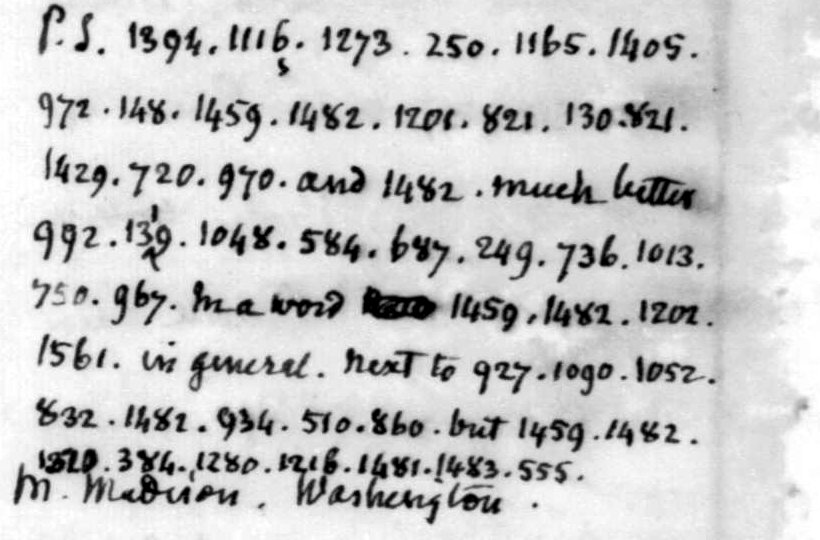
\includegraphics[width=0.85\textwidth]{figures/fig1_postscript_loc.jpg}
\caption{The coded postscript of 30 August 1808. A pencil \emph{s} beneath the second group, \grp{1116}, is a decode begun and abandoned in Washington. Library of Congress, Manuscript Division, James Madison Papers (public domain).}
\label{fig:ps}
\end{figure}

\emph{Founders Online} \citep{Founders:3466} prints the groups as follows; the manuscript differs in two of them (Section~\ref{sec:corr}):

\begin{quote}\small\grp{
1394. 1116. 1273. 250. 1165. 1405. \\
970. 148. 1459. 1482. 1201. 821. 130. 821. \\
1429. 720. 970. and 1482. much better \\
992. 1319. 1048. 584. 687. 249. 736. 1013. \\
750. 967. In a word 1459. 1482. 1202. \\
1561. in general. Next to 927. 1090. 1052. \\
832. 1482. 934. 510. 860. but 1459. 1482. \\
1320. 384. 1280. 1218. 1481. 1483. 555.}
\end{quote}

Six clear words (\emph{and}, \emph{much better}, \emph{In a word}, \emph{in general}, \emph{Next to}, \emph{but}) are left in the open, a habit of Armstrong's that itself constrains the reading.

\section{The code}\label{sec:code}

Armstrong's despatches from Paris between 1804 and 1810 use a single large code in which \grp{972} = \emph{the}. Weber notes some forty letters in it among the Despatches from United States Ministers to France (National Archives, Record Group 59, microcopy M34, rolls 13--14; \citealp{Weber:1979}). It is not the code of Armstrong's letter of 20 February 1808, a distinct system that remains unsolved and is outside the scope of this paper. As recovered, the code has the following structure.

\paragraph{Range and units.} Groups run from 1 to about 1600, with one recorded value at 1687. Each stands for a whole word (\emph{Emperor} \grp{32}, \emph{Spain} \grp{326}, \emph{Minister} \grp{61}), a syllable (\emph{con} \grp{470}, \emph{tion} \grp{352}, \emph{ness} \grp{832}), or a single letter (\emph{s} \grp{1116}, \emph{n} \grp{821}, \emph{d} \grp{1001}). Names are spelt in syllables: \emph{Gu-sta-va-us}, \emph{Et-ru-ria}, \emph{Y-ru-jo}, \emph{Dan-ish}, \emph{O-mea-ly}.

\paragraph{Layout.} The vocabulary is laid out in many short alphabetical runs rather than one sequence. Groups up to about 128 form a run of words (\emph{character}, \emph{circumstance}, \emph{commerce} \ldots\ \emph{Minister} \ldots\ \emph{these}, \emph{thousand}, \emph{toward} \ldots\ \emph{without}, \emph{yesterday}); 130 to about 411 a second, itself in sub-runs (\emph{America}, \emph{between}, \emph{business}, \emph{confide}, \emph{contrary}, \emph{country} \ldots\ \emph{Prince}, \emph{Queen}, \emph{reason}, \emph{report}, \emph{Russia}, \emph{second}, \emph{secret} \ldots\ \emph{which}, \emph{whom}, \emph{word}, \emph{would}, \emph{your}); above 417 the syllables come in blocks that restart the alphabet every few dozen numbers (\grp{1201} \emph{a} \ldots\ \grp{1230} \emph{c}; \grp{1268} \emph{ed} \ldots\ \grp{1298} \emph{ex}; \grp{1405} \emph{be} \ldots\ \grp{1443} \emph{good}; the 1500s \emph{fa} \ldots\ \emph{man} \ldots\ \emph{now}). Table~\ref{tab:runs} lists the runs that the recovered groups define. Within a run the order is alphabetical, which is what allows an unknown group to be pinned between known neighbours: \grp{148} lies between \grp{146} \emph{confide} and \grp{151} \emph{contrary}, and the postscript needs \emph{consul}.

\begin{table}
\tbl{Alphabetical runs of the code as defined by the recovered groups. A run boundary is placed wherever consecutive known groups break alphabetical order, so a single misread value can split a run; only runs with six or more known groups are listed (33 of 102 detected), and doubtful readings carry a query.}
{\begin{tabular}{@{}rrrll@{}}
\toprule
from & to & known groups & first & last \\
\midrule
13 & 112 & 17 & \emph{character} & \emph{ver} \\
130 & 203 & 20 & \emph{America} & \emph{timate} \\
207 & 240 & 7 & \emph{Madrid} & \emph{roc} \\
244 & 279 & 15 & \emph{October} & \emph{tion} \\
282 & 293 & 8 & \emph{proper} & \emph{ti} \\
305 & 316 & 6 & \emph{Russia} & \emph{should} \\
319 & 339 & 7 & \emph{6th}? & \emph{tend} \\
341 & 372 & 15 & \emph{temp} & \emph{view} \\
377 & 411 & 16 & \emph{under} & \emph{z} \\
479 & 532 & 22 & \emph{cause} & \emph{vot} \\
541 & 560 & 6 & \emph{offer} & \emph{rent} \\
578 & 615 & 19 & \emph{t} & \emph{vin} \\
636 & 669 & 15 & \emph{mp} & \emph{put} \\
721 & 759 & 14 & \emph{b} & \emph{des} \\
760 & 779 & 7 & \emph{de} & \emph{ea} \\
808 & 854 & 19 & \emph{able} & \emph{such} \\
860 & 891 & 15 & \emph{ly} & \emph{yoke} \\
914 & 944 & 13 & \emph{gu} & \emph{vol} \\
945 & 974 & 15 & \emph{on} & \emph{tho} \\
981 & 989 & 7 & \emph{s} & \emph{sue} \\
1001 & 1028 & 13 & \emph{d} & \emph{il} \\
1041 & 1048 & 6 & \emph{feat} & \emph{fi(ed)} \\
1050 & 1075 & 9 & \emph{fi} & \emph{refu} \\
1089 & 1154 & 26 & \emph{im} & \emph{vy} \\
1203 & 1222 & 7 & \emph{a} & \emph{ce} \\
1223 & 1231 & 6 & \emph{are} & \emph{tical} \\
1246 & 1257 & 8 & \emph{col} & \emph{duct} \\
1272 & 1286 & 8 & \emph{eight} & \emph{p}? \\
1287 & 1324 & 14 & \emph{equal} & \emph{plo} \\
1348 & 1383 & 13 & \emph{broa} & \emph{rep} \\
1428 & 1500 & 36 & \emph{but} & \emph{lesia} \\
1501 & 1565 & 23 & \emph{Eu} & \emph{mil} \\
1566 & 1585 & 6 & \emph{mi} & \emph{now} \\
\bottomrule
\end{tabular}}
\label{tab:runs}
\end{table}

\paragraph{Homophones.} Common elements have several groups: \emph{re} is \grp{555}, \grp{561}, \grp{562}, \grp{869} and \grp{871} among others; \emph{al} is \grp{420} and \grp{817}. One trap in the pencil: where the clerk wrote a whole word over the first of its groups, he marked the continuation groups with a dash. \grp{1394} carries such a dash under \emph{Etruria} and \emph{Yrujo} and was at first taken for a null; it is \emph{ru}, and it opens the postscript.

\section{Sources and method}\label{sec:method}

\subsection{Two kinds of known plaintext}

The first source is the one Tomokiyo used: Armstrong's letter of 4 May 1806, whose decode is preserved with it, giving 227 values, graded here \textbf{C} (confirmed by known plaintext). The second is new. The despatches Armstrong sent to the Department of State were decoded on receipt, and in the bound despatch books, microfilmed as M34 \citep{NARA:M34}, the clerk's decode is written in pencil above each group of the coded passages (Figure~\ref{fig:pencil}). On roll 13, which covers November 1804 to December 1807, a long political despatch of October 1806 (frames 0192--0201) is decoded in this way throughout, and shorter passages elsewhere on the roll add more: frame 0190, a despatch of 20 July 1806 on the Franco-Russian peace, gives \emph{like}, \emph{last}, \emph{night}, \emph{about}, \emph{look}. Values read from these pencil decodes are graded \textbf{H} when the pencil is legible and \textbf{M} when it is doubtful.

\begin{figure}
\centering
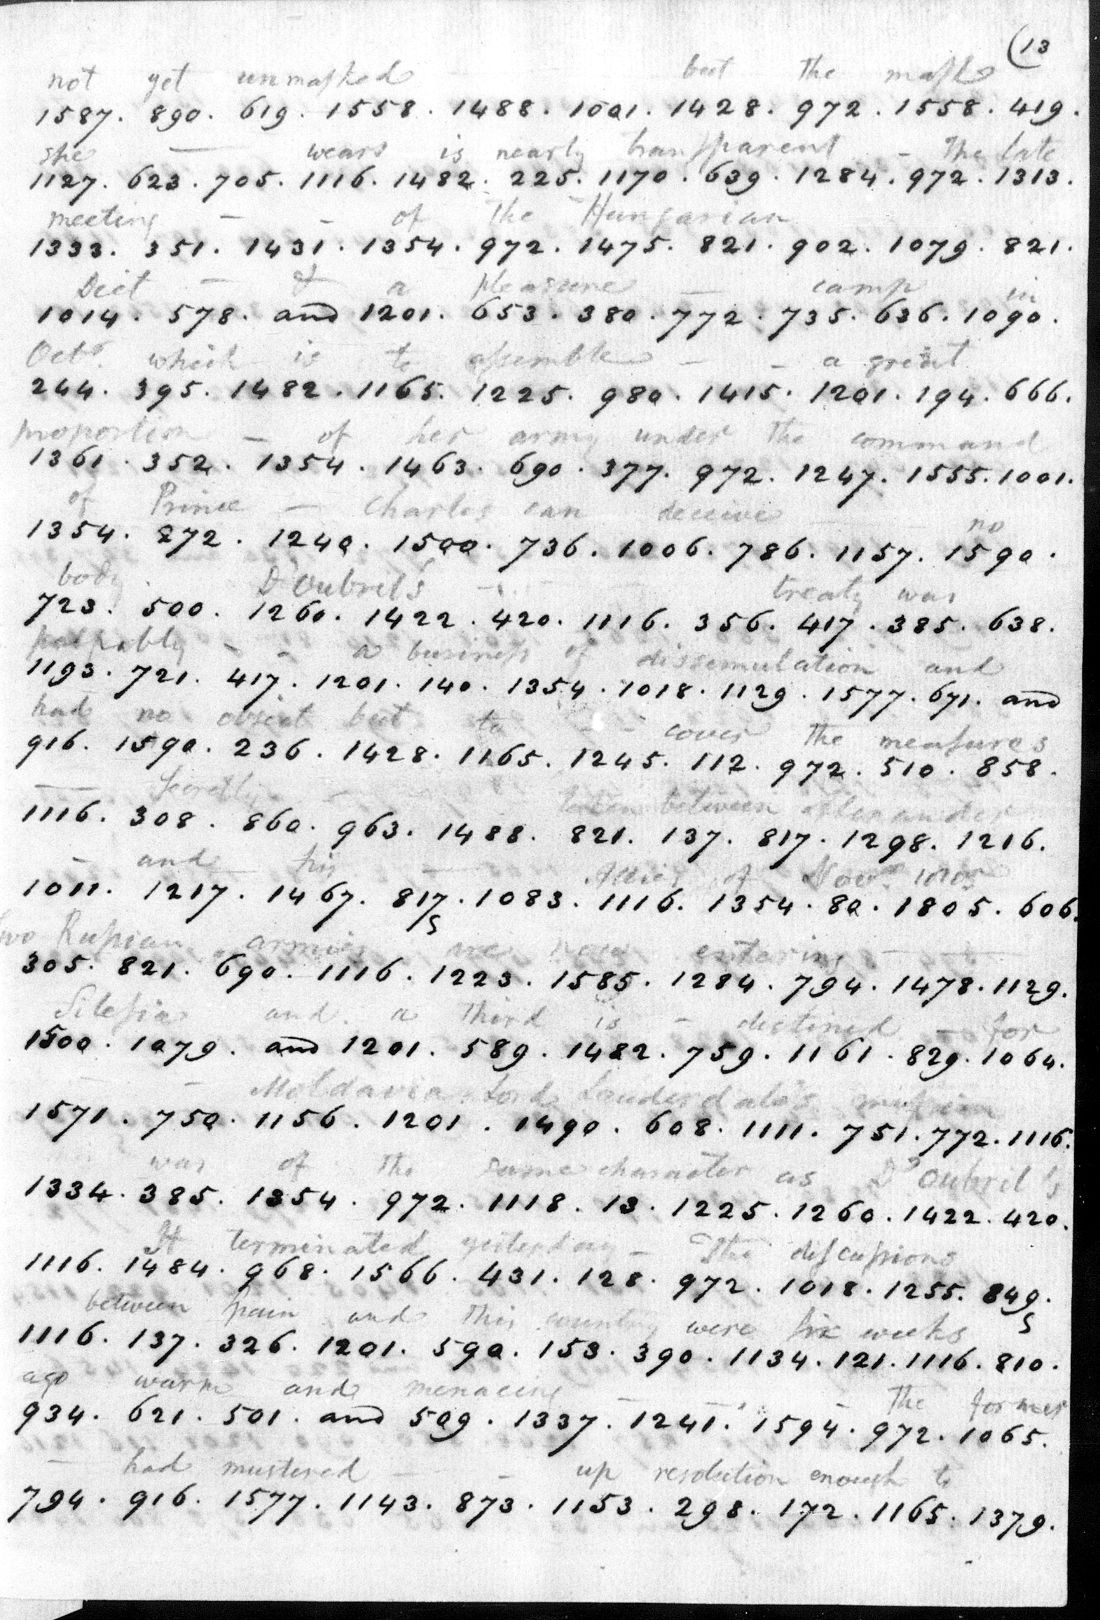
\includegraphics[width=0.7\textwidth]{figures/fig2_m34_roll13_frame0200.jpg}
\caption{M34 roll 13, frame 0200: a page of Armstrong's despatch of October 1806 with the State Department clerk's pencil decode above each group. Dashes mark groups whose value was written over the preceding group. National Archives, Record Group 59, Despatches from United States Ministers to France (unrestricted).}
\label{fig:pencil}
\end{figure}

\subsection{Finding the annotated frames}

Reading 393 frames of manuscript for faint pencil is slow by eye, and we tried to shorten it with an image score. Each frame is reduced to grey; pixels darker than 100 of 255 are taken as ink and dilated by a few pixels; the score is the proportion of the remaining pixels that are mid-grey, that is, faint marks not adjacent to ink. The score was used during the work as a triage aid alongside browsing, and the annotated frames were confirmed by eye. Rerun afterwards over the whole roll, it does not perform as a detector, and we report that rather than the impression it gave at the time. The raw score is dominated by grey blank leaves and dark bleed-through: 73 of 392 frames score above the first page of the October despatch (frame 0192) and 94 above frame 0200, whose pencil is the densest on the roll. Defining ``grey'' relative to each page's own background and counting only the interlinear band within twenty pixels of ink, and only on pages with a bright background, improves it: the first page of the October despatch then ranks third of 392, and the 4 May 1806 letter, which carries its own pencil decode, ranks second under a whole-page version of the same score. But the later pages of the despatch (0196--0201), where the pencil is fainter and the page darker, still rank in the bottom third under every variant, behind pages with no pencil at all. A score of this kind can find the first, heavily annotated page of a decoded despatch and so shorten the search; it cannot be relied on to find every annotated page, and we would not now claim more for it. The scores of all frames under each variant are released with the table.

\subsection{Harvesting, grading, merging}

Each annotated frame was cropped into thirds, contrast-enhanced and read group by group; every number--value pair was recorded with its frame and line and a confidence grade. Groups seen on several frames were cross-checked: \grp{1555} \emph{man}, for instance, appears on frames 0195 and 0200 (``the command of Prince Charles'', ``man''). 582 pairs were harvested, 399 graded H and 183 M, covering 533 distinct groups.

A script merges the three layers, ranking readings H $>$ C $>$ M $>$ inferred, and renders any coded passage with unknown and doubtful groups flagged. The merged table has 607 entries: 374 rest on legible pencil, 62 on the 4 May 1806 plaintext alone, 153 on doubtful pencil, and 18 are inferences (grade \textbf{I}) from context checked against the alphabetical slot. Finally the letter of 22 February 1808, also coded in the 972 system and also unread, was decoded with the same table as an independent control. It shares no groups of interest with the known-plaintext letter and reads coherently: ``The ruin of Gustavus is at last resolved. Russia is to seize Finland, while France \& Denmark take possession of Sweden \ldots\ the Danish Minister was this morning pouring out his complaints to me upon this subject.'' It fixes \emph{ru}, \emph{ish} and \emph{Russia} (\grp{305}), which the postscript needs, and shows two probable single-digit slips of the microfilm hand (\grp{631} \emph{wise} for \grp{651} \emph{plain}; \grp{916} \emph{had} for \grp{921} \emph{have}) and one anomaly (\grp{946}, \emph{on} in the 1806 letter, must be \emph{Gu} in \emph{Gustavus}, where \grp{914} is \emph{gu} elsewhere; a homophone or a slip).

\subsection{Collation}

The Library of Congress image of the postscript was enlarged and every group compared with the \emph{Founders} text (Section~\ref{sec:corr}).

\section{The reading}\label{sec:reading}

\begin{quote}
Russel ought to be the consul: he is an American by birth, and is much better qualified than any other candidate. In a word, he is above men in general. Next to him in fitness is O'Mealy, but he is, like Warden, an Irishman.
\end{quote}

Table~\ref{tab:ps} gives the 49 groups with value, grade and source. Thirty-four rest on legible pencil (H), three on the 1806 plaintext (C), eleven on slot inference (I), and one, the last, is a probable slip. All eleven inferred values fit their alphabetical slot: \grp{1273} \emph{el} between \grp{1272} \emph{eight} and \grp{1279} \emph{Emp}; \grp{250} \emph{ought} between \grp{249} \emph{other} and \grp{252} \emph{own}; \grp{148} \emph{consul} between \grp{146} \emph{confide} and \grp{151} \emph{contrary}; \grp{130} \emph{America} at a run boundary after \grp{128} \emph{yesterday} and before \grp{137} \emph{between}; \grp{720} \emph{bir} between \grp{719} \emph{Ba} and \grp{723} \emph{bo}; \grp{992} \emph{qua} before \grp{993} \emph{qui}; \grp{1048} \emph{fi(ed)} in the \emph{fi} block 1046--1052; \grp{1202} \emph{above} between \grp{1201} \emph{a} and \grp{1209} \emph{Agent}; \grp{1052} \emph{fit} between \grp{1050} \emph{fi} and \grp{1064} \emph{for}; \grp{384} \emph{Ward} between \grp{383} \emph{w} and \grp{385} \emph{was}; \grp{1483} \emph{ish} between \grp{1482} \emph{is} and \grp{1484} \emph{it}. The February letter confirms \emph{ru} (\emph{ru-in}) and \emph{ish} (\emph{Dan-ish}) independently, and \emph{ru} is also read from the pencil under \emph{Et-ru-ria} (frame 0201) and \emph{Y-ru-jo} (frame 0194).

\begin{table}
\tbl{The 49 groups of the postscript. Grades: H legible pencil decode on M34 roll 13 (frame given); C the 4 May 1806 known plaintext; I inferred from context and the alphabetical slot. Group 49 is discussed in Section~\ref{sec:corr}.}
{\small\begin{tabular}{@{}rlll@{\qquad}rlll@{}}
\toprule
\# & group & value & grade, source & \# & group & value & grade, source \\
\midrule
1 & 1394 & \emph{ru} & H 0194, 0201 & 26 & 1013 & \emph{di} & C \\
2 & 1116 & \emph{s} & H 0200 & 27 & 750 & \emph{da} & H 0200 \\
3 & 1273 & \emph{el} & I & 28 & 967 & \emph{te} & H 0200 \\
4 & 250 & \emph{ought} & I & 29 & 1459 & \emph{he} & H 0200 \\
5 & 1165 & \emph{to} & H 0200 & 30 & 1482 & \emph{is} & H 0200 \\
6 & 1405 & \emph{be} & H 0201 & 31 & 1202 & \emph{above} & I \\
7 & 972 & \emph{the} & H 0200 & 32 & 1561 & \emph{men} & H 0201 \\
8 & 148 & \emph{consul} & I & 33 & 927 & \emph{him} & C \\
9 & 1459 & \emph{he} & H 0200 & 34 & 1090 & \emph{in} & H 0200 \\
10 & 1482 & \emph{is} & H 0200 & 35 & 1052 & \emph{fit} & I \\
11 & 1201 & \emph{a} & H 0200 & 36 & 832 & \emph{ness} & H 0196 \\
12 & 821 & \emph{n} & H 0200 & 37 & 1482 & \emph{is} & H 0200 \\
13 & 130 & \emph{America} & I & 38 & 934 & \emph{o} & H 0193 \\
14 & 821 & \emph{n} & H 0200 & 39 & 510 & \emph{mea} & H 0200 \\
15 & 1429 & \emph{by} & H 0200 & 40 & 860 & \emph{ly} & H 0200 \\
16 & 720 & \emph{bir} & I & 41 & 1459 & \emph{he} & H 0200 \\
17 & 970 & \emph{th} & H 0201 & 42 & 1482 & \emph{is} & H 0200 \\
18 & 1482 & \emph{is} & H 0200 & 43 & 1320 & \emph{like} & H 0190 \\
19 & 992 & \emph{qua} & I & 44 & 384 & \emph{Ward} & I \\
20 & 1319 & \emph{li} & C & 45 & 1280 & \emph{en} & H 0201 \\
21 & 1048 & \emph{fi(ed)} & I & 46 & 1216 & \emph{an} & H 0200 \\
22 & 584 & \emph{than} & H 0194 & 47 & 1481 & \emph{ir} & H 0195, 0201 \\
23 & 687 & \emph{any} & H 0200 & 48 & 1483 & \emph{ish} & I \\
24 & 249 & \emph{other} & H 0201 & 49 & 555 & \emph{[man]} & slip for 1555, H 0195, 0200 \\
25 & 736 & \emph{can} & H 0200 & & & & \\
\bottomrule
\end{tabular}}
\label{tab:ps}
\end{table}

\paragraph{Historical sense.} \emph{Russel}, spelt \emph{Ru-s-el}, is most probably Jonathan Russell of Providence, Rhode Island (1771--1832), a merchant in the European trade whom Madison did appoint charg\'e d'affaires at Paris when Armstrong left in 1810; the identification is inferential, since no other document places him in France in 1808. David Bailie Warden (1772--1845), born in County Down, a United Irishman exiled in 1799 and naturalised American, was Armstrong's secretary of legation and the front-runner for the vacant consulate; he got it, Armstrong removed him in 1810, and when Madison reinstated him in 1811 Armstrong protested that Warden was ``without a single grain of attachment to the U.S.'' and asked whether ``our own country furnish[es] no native citizen'' for the post (3 March 1811). The postscript shows the same animus three years earlier and names its cause. Michael O'Mealy was a Baltimore merchant resident in France since 1793 (\emph{Papers of James Madison, Secretary of State Series} 10:497 n.~2). That Armstrong reserved this ranking for code, while treating Warden neutrally in clear, is the pattern of use one expects of a diplomatic code: the text is ordinary, and the secret is an opinion about persons.

\section{Corrections to the printed transcription, and one doubt}\label{sec:corr}

\emph{Founders} prints \grp{970.} at the start of the second line where the manuscript has \grp{972.} (\emph{the}); \grp{970} is \emph{th}, which the sentence cannot use there. \emph{Founders} prints \grp{1218} in the last line; the manuscript reads \grp{1216} (\emph{an}), which is also what the sentence requires. A pencil \emph{s} below \grp{1116} on the Library of Congress copy shows that a reader in Washington began, and abandoned, a decode.

The final group is \grp{555} both in \emph{Founders} and in the manuscript. \grp{555} is \emph{re} (frame 0195: \emph{sco-re}), which makes no sense after \emph{Irish}, whereas \grp{1555} is \emph{man}. The reading \emph{Irishman} assumes Armstrong dropped a digit; the alternative, that the postscript breaks off with ``an Irish re\ldots'', is recorded for completeness. Of 49 groups, 48 are therefore determined and one is a probable slip.

\section{Discussion}\label{sec:disc}

Three points generalise beyond this letter.

First, the receiving department's working copies are a known-plaintext source of a different order from a single decoded letter. A clerk decoding a despatch writes every value, common and rare alike, and the pencil survives microfilming well enough to be read at the resolution of the National Archives' catalogue images. Any American code of the period whose despatches were decoded on receipt can probably be recovered in the same way; Weber's survey \citeyearpar{Weber:1979} lists the candidates.

Second, the alphabetical one-part layout turns a partial table into a nearly complete one. Once the runs are identified, an unknown group has only a handful of possible values, and context chooses among them. The grading scheme (H, C, M, I) keeps the two kinds of knowledge apart, so that a reader can see which values rest on ink and which on inference.

Third, the printed transcription had two wrong digits in 49 groups. Collation with the manuscript image is not optional for coded text, where a single digit changes the word.

What remains is the rest of the 972 corpus. Thirty-seven further frames of roll 13 with coded passages were downloaded but have not been read group by group (0011--0012, 0016--0017, 0021, 0027, 0034--0035, 0058--0059, 0096--0097, 0109--0110, 0121--0122, 0140--0143, 0150--0151, 0160, 0188--0189, 0191, 0223--0225, 0232--0238, 0289); several carry pencil and may turn the eleven inferred values of the postscript into read ones. Roll 14 (1808--1810) has not been examined beyond the two 1808 letters used here. Some forty coded Armstrong despatches can now be read with the table.

\section{Conclusion}

The coded postscript of 30 August 1808 is read in full, from a code reconstructed largely out of the State Department's own pencil decodes rather than from any surviving code book. The postscript itself is a private ranking of candidates for the Paris consulate. The method, harvesting the receiving department's interlinear pencil decodes with a per-value grade and exploiting the alphabetical layout of a one-part code, is applicable to the other coded American despatches of the period; the image score we tried for locating the pencil is a partial aid at best, and the honest advice is to page through the roll.

\section*{Data availability statement}

The 607-entry code table with a frame reference for every pencil reading, the harvested pairs, the decoder and the image-scoring script are deposited in a public repository; the location is withheld for review and will be given in the published version.

% Acknowledgements, disclosure statement and notes on contributor: non-anonymous version only (see titlepage.tex).

\bibliographystyle{tfcad}
\bibliography{refs}

\appendix
\section{The recovered code table}\label{app:table}

Groups with a value in the merged table, 607 entries. Grade H: legible pencil decode, with the roll 13 frame(s); C: the 4 May 1806 known plaintext; M: doubtful pencil; I: inferred. Readings carrying a query or an asterisk are the harvester's own doubt marks and are retained.

{\small
% entries: 607
\begin{longtable}{@{}rlll@{}}
\toprule group & value & grade & source \\ \midrule \endhead
1 & circumstance & H & 0195, 0201 \\
4 & commerce & H & 0201 \\
5 & communica & H & 0195 \\
13 & character & H & 0200 \\
14 & commit & C & 4 May 1806 \\
16 & condition & H & 0200 \\
21 & could & C & 4 May 1806 \\
26 & Denmark & I & inferred \\
27 & difficult & H & 0195 \\
32 & Emperor & H & 0201 \\
36 & Germany & H & 0199 \\
41 & however & H & 0193 \\
61 & minister & H & 0193 \\
64 & Monarch & H & 0195 \\
91 & particular & M & 0195 \\
103 & these & H & 0194 \\
105 & thought & H & 0194 \\
106 & thousand & H & 0201 \\
109 & toward & C & 4 May 1806 \\
112 & ver & H & 0200 \\
115 & US & H & 0195 \\
116 & unless & M & 0201 \\
121 & week & H & 0200 \\
127 & without & H & 0201 \\
128 & yesterday & H & 0200 \\
130 & America & M & alpha(127without|137between)+PS \\
137 & between & H & 0200, 0201 \\
140 & business & H & 0200 \\
146 & confide & C & 4 May 1806 \\
148 & consul & M & alpha(146confide,151contrary)+PS \\
151 & contrary & H & 0201 \\
153 & country & H & 0199, 0200 \\
156 & demand & H & 0201 \\
157 & depend & H & 0201 \\
158 & design & H & 0198 \\
166 & either & H & 0200 \\
170 & England & H & 0193, 0194 \\
174 & Europe & M & 0199 \\
175 & ex* & C & 4 May 1806 \\
187 & Florida & C & 4 May 1806 \\
190 & French & H & 0201 \\
191 & general & H & 0198 \\
193 & govern & H & 0193p3-1,0193p3-3 \\
199 & hither & M & 0195 \\
203 & timate & H & 0201 \\
207 & Madrid & H & 0194 \\
220 & money & H & 0201 \\
225 & near & M & 0199 \\
228 & never & H & 0201 \\
231 & new & H & 0200 \\
236 & object & H & 0200 \\
240 & roc & H & 0195 \\
244 & October & H & 0200 \\
249 & other & H & 0201 \\
250 & ought & I & inferred \\
252 & own & H & 0198 \\
254 & Paris & C & 4 May 1806 \\
255 & part & H & 0198 \\
256 & peace & H & 0198 \\
257 & people & H & 0201 \\
264 & Portugal & H & 0201 \\
268 & power & H & 0199 \\
269 & present & H & 0201 \\
272 & Prince & H & 0200 \\
273 & princi & M & 0201 \\
277 & probab & H & 0195 \\
279 & tion & M & 0194 \\
282 & proper & H & 0195 \\
284 & pub & H & 0201 \\
286 & Queen & H & 0201 \\
288 & rather & H & 0195 \\
289 & ration & H & 0194 \\
290 & reason & C & 4 May 1806 \\
291 & recei & M & 0195 \\
293 & ti & M & 0200 \\
295 & report & M & 0196 \\
297 & resolve & I & inferred \\
301 & tri & H & 0194 \\
305 & Russia & H & 0200 \\
307 & second & H & 0201 \\
308 & secret & H & 0200 \\
309 & Sept & M & 0199 \\
312 & set & H & 0199 \\
316 & should & H & 0198 \\
319 & 6th? & M & 0193 \\
322 & some & H & 0194 \\
323 & sp & M & 0198 \\
326 & Spain & H & 0200 \\
330 & station & C & 4 May 1806 \\
337 & ta & M & 0194 \\
339 & tend & M & 0198 \\
340 & ten & M & 0198 \\
341 & temp & C & 4 May 1806 \\
344 & there & H & 0201 \\
345 & thing & H & 0193 \\
346 & thirty & H & 0201 \\
348 & three & H & 0201 \\
350 & time & H & 0195 \\
351 & tin & H & 0200 \\
352 & tion & H & 0200 \\
353 & tion & M & 0199 \\
356 & trea & H & 0200 \\
358 & trust & C & 4 May 1806 \\
360 & tude & M & 0193p3-2 \\
369 & very & H & 0201 \\
370 & vest & C & 4 May 1806 \\
372 & view & H & 0200 \\
377 & under & H & 0200 \\
379 & upon & H & 0194 \\
380 & ur & H & 0200 \\
383 & w & H & 0195 \\
384 & ward & I & inferred \\
385 & was & H & 0200 \\
386 & way & H & 0201 \\
390 & were & H & 0200 \\
393 & when & H & 0198 \\
395 & which & H & 0200 \\
396 & while & I & inferred \\
397 & whom & H & 0194 \\
402 & word & H & 0201 \\
405 & would & H & 0200, 0201 \\
410 & your & C & 4 May 1806 \\
411 & z & H & 0195 \\
415 & you & H & 0199 \\
417 & y & H & 0200 \\
418 & ose & H & 0200 \\
419 & k & H & 0198 \\
420 & al & H & 0200 \\
424 & affair & H & 0194 \\
425 & after & H & 0195 \\
430 & appear & H & 0200, 0201 \\
432 & tion & H & 0201 \\
444 & Ber & M & 0200 \\
447 & better & H & 0201 \\
459 & cure & M & 0195 \\
460 & cy & H & 0194 \\
465 & count & C & 4 May 1806 \\
468 & con & M & 0194 \\
470 & con & H & 0200 \\
471 & con & C & 4 May 1806 \\
475 & circum & M & 0195 \\
477 & change & H & 0201 \\
479 & cause & H & 0201 \\
484 & den & M & 0193 \\
486 & diffe & H & 0201 \\
500 & dy & H & 0200 \\
501 & m & H & 0200 \\
502 & made & H & 0201 \\
505 & march & H & 0201 \\
507 & mark & H & 0199 \\
508 & may & H & 0193p3-2 \\
509 & me & H & 0200 \\
510 & mea & H & 0200 \\
511 & mean & H & 0195 \\
512 & media & M & 0190 \\
514 & ment & H & 0200 \\
516 & might & M & 0195 \\
518 & mis & M & 0201 \\
520 & mod & M & 0198 \\
523 & most & C & 4 May 1806 \\
526 & much & H & 0200 \\
529 & my & H & 0199 \\
530 & order & H & 0193 \\
532 & vot & M & 0195 \\
533 & mote & H & 0200 \\
537 & out & H & 0199 \\
541 & offer & H & 0194 \\
550 & one & H & 0200 \\
555 & re & H & 0195 \\
558 & relat & M & 0199 \\
559 & rem & H & 0193 \\
560 & rent & H & 0195 \\
561 & re & H & 0200 \\
562 & re & M & 0199 \\
570 & roa & M & 0195 \\
576 & ery & M & 0201 \\
577 & tack & M & 0194 \\
578 & t & H & 0200 \\
579 & take & M & 0200 \\
582 & ted & H & 0199 \\
584 & than & H & 0194 \\
585 & their & H & 0200 \\
586 & then & H & 0194 \\
587 & they & H & 0200 \\
589 & third & H & 0200 \\
590 & this & H & 0199 \\
591 & those & H & 0193bot \\
593 & thro & H & 0201 \\
603 & tune & H & 0200 \\
605 & twe & M & 0194 \\
606 & Two & M & 0201 \\
607 & ty & H & 0201 \\
608 & va & C & 4 May 1806 \\
609 & vail & H & 0200 \\
611 & ved & H & 0193, 0201 \\
615 & vin & C & 4 May 1806 \\
618 & ul & H & 0200 \\
619 & un & H & 0200 \\
621 & ar & M & 0200 \\
623 & we & M & 0196 \\
626 & who & H & 0200 \\
627 & whole & M & 0198 \\
629 & v & C & 4 May 1806 \\
630 & will & H & 0199 \\
631 & wise & C & 4 May 1806 \\
632 & with & H & 0201 \\
633 & Ta? & M & 0194 \\
636 & mp & H & 0201 \\
639 & pa* & C & 4 May 1806 \\
644 & pen & M & 0194 \\
646 & per & H & 0201 \\
647 & ph & H & 0201 \\
651 & plain & H & 0201 \\
653 & pleas & H & 0200 \\
655 & plish & M & 0195 \\
658 & point & H & 0194 \\
659 & port & H & 0201 \\
662 & pres & M & 0198 \\
664 & pro & H & 0200 \\
665 & pro & H & 0200 \\
667 & pros & M & 0201 \\
669 & put & C & 4 May 1806 \\
671 & lation & M & 0200 \\
674 & ledge & H & 0201 \\
676 & letter & H & 0199 \\
679 & look & H & 0190 \\
687 & any & H & 0200 \\
690 & army & H & 0200 \\
692 & ary & C & 4 May 1806 \\
698 & aid & H & 0195 \\
702 & ance & H & 0198 \\
704 & ap & H & 0195 \\
706 & ard & M & 0201 \\
716 & been & H & 0199 \\
718 & bat & H & 0201 \\
719 & Ba & M & 0200 \\
720 & bir & I & inferred \\
721 & b & M & 0193 \\
723 & bo & H & 0200 \\
734 & Ca & H & 0200 \\
735 & cam & H & 0201 \\
736 & can & H & 0200 \\
741 & ce & H & 0200, 0201 \\
742 & cei & M & 0198 \\
745 & chan & H & 0200 \\
747 & ck & H & 0201 \\
750 & da & H & 0200 \\
752 & dan & H & 0195 \\
753 & day & H & 0193, 0199 \\
758 & dep & I & inferred \\
759 & des & H & 0200, 0201 \\
760 & de & M & 0195 \\
761 & did & H & 0194 \\
765 & does & H & 0195 \\
769 & dress & M & 0195 \\
772 & e & H & 0200 \\
773 & ea & M & 0198 \\
779 & ea & M & 0198 \\
781 & ct & H & 0195 \\
784 & ef & H & 0193 \\
786 & ei & H & 0200 \\
790 & rence & H & 0201 \\
792 & p & M & 0198 \\
793 & er & M & 0195 \\
794 & er & H & 0200 \\
795 & ri & M & 0195 \\
798 & est & H & 0195 \\
801 & about & H & 0190 \\
802 & ab & M & 0200 \\
803 & ac & H & 0201 \\
804 & act & H & 0198 \\
805 & add & H & 0201 \\
808 & able & H & 0195 \\
810 & ag & M & 0200 \\
811 & age & H & 0198 \\
817 & al & H & 0200 \\
819 & also & H & 0195 \\
821 & n & H & 0200 \\
822 & nal & H & 0201 \\
825 & nce & I & inferred \\
827 & ne & M & 0198 \\
829 & ned & H & 0200 \\
832 & ness & H & 0196 \\
835 & night & H & 0190 \\
840 & none & H & 0195 \\
844 & nty & C & 4 May 1806 \\
848 & side & M & 0194 \\
849 & sions & M & 0200 \\
850 & sive & H & 0201 \\
853 & state & M & 0199 \\
854 & such & H & 0195 \\
855 & pal & M & 0201 \\
856 & suf & C & 4 May 1806 \\
857 & sum & H & 0201 \\
858 & sures & H & 0200 \\
859 & sy & H & 0200 \\
860 & ly & H & 0200 \\
864 & pro & C & 4 May 1806 \\
865 & quest & H & 0201 \\
867 & ran & H & 0194 \\
868 & rd & C & 4 May 1806 \\
869 & re* & C & 4 May 1806 \\
871 & re & M & 0200 \\
872 & rec & H & 0199 \\
873 & red & M & 0193p3-2 \\
876 & ria & M & 0201 \\
882 & ro & H & 0201 \\
885 & urs & M & 0195 \\
888 & x & H & 0200 \\
890 & yet & H & 0200 \\
891 & yoke & H & 0200 \\
899 & us & H & 0200 \\
901 & ga & H & 0198 \\
903 & ged & M & 0195 \\
907 & give & H & 0201 \\
910 & particular & C & 4 May 1806 \\
914 & gu & H & 0198 \\
916 & had & H & 0200 \\
917 & half & I & inferred \\
921 & have & H & 0200 \\
922 & hea & H & 0201 \\
925 & here & H & 0195 \\
926 & high & C & 4 May 1806 \\
927 & him & C & 4 May 1806 \\
932 & how & H & 0198 \\
934 & o & H & 0193, alpha+0200 \\
939 & sue & H & 0201 \\
943 & upon & I & inferred \\
944 & vol & M & 0199 \\
945 & on & H & 0201 \\
946 & on & C & 4 May 1806 \\
947 & only & H & 0195 \\
951 & ose & H & 0201 \\
953 & ou & C & 4 May 1806 \\
963 & ta & H & 0200 \\
964 & tain & M & 0195 \\
965 & tal & H & 0195 \\
967 & te & H & 0200 \\
968 & ter & H & 0200, 0201 \\
970 & th & H & 0201 \\
971 & that & H & 0200 \\
972 & the & H & 0200 \\
973 & them & H & 0200 \\
974 & tho & C & 4 May 1806 \\
975 & Sa & H & 0200 \\
976 & sal & H & 0201 \\
977 & scrip & M & 0201 \\
979 & sel & M & 0200 \\
980 & sem & M & 0200 \\
981 & s & M & 0198 \\
983 & so & H & 0200, 0201 \\
985 & sta & C & 4 May 1806 \\
986 & sti & H & 0198 \\
987 & stre & M & 0201 \\
988 & sub & H & 0201 \\
989 & sue & M & 0194 \\
991 & answ & M & 0195 \\
992 & qua & I & inferred \\
993 & qui & M & 0201 \\
1001 & d & H & 0200 \\
1005 & de & H & 0200 \\
1006 & dec & H & 0200 \\
1009 & del & M & 0194 \\
1010 & dent & C & 4 May 1806 \\
1013 & di & C & 4 May 1806 \\
1014 & die & M & 0200 \\
1017 & din & M & 0194 \\
1018 & dis & H & 0200 \\
1020 & do & H & 0195 \\
1024 & dom & H & 0201 \\
1027 & dra & M & 0201 \\
1028 & il & M & 0200 \\
1031 & Du & H & 0195 \\
1032 & f & M & 0201 \\
1034 & fact & H & 0196 \\
1039 & fav & M & 0195 \\
1040 & fee & M & 0193 \\
1041 & feat & M & 0198 \\
1042 & fect & H & 0193 \\
1044 & fer & M & 0193p3-2 \\
1045 & few & H & 0199 \\
1046 & fi & H & 0194 \\
1048 & fi(ed) & I & inferred \\
1050 & fi & M & 0201 \\
1052 & fit & M & alpha(1046fi,1050fi,1064for)+PS \\
1062 & fol & M & 0199 \\
1064 & for & H & 0200 \\
1065 & former & H & 0200 \\
1069 & France & H & 0201 \\
1070 & fre & H & 0194 \\
1071 & fri & C & 4 May 1806 \\
1075 & refu & M & 0201 \\
1078 & I & H & 0201 \\
1079 & i* & C & 4 May 1806 \\
1080 & fin & C & 4 May 1806 \\
1082 & rt & I & inferred \\
1083 & ie & H & 0198, 0201 \\
1087 & ig & H & 0201 \\
1088 & mil & H & 0201 \\
1089 & im & H & 0195 \\
1090 & in & H & 0200 \\
1093 & ise & M & 0194 \\
1095 & ju & H & 0198 \\
1098 & King & H & 0201 \\
1099 & lan & H & 0198, 0201 \\
1116 & s & H & 0200 \\
1118 & same & H & 0200 \\
1120 & sco & H & 0195 \\
1121 & se & H & 0200 \\
1123 & self & H & 0199 \\
1124 & sen & M & 0194 \\
1125 & sent & H & 0201 \\
1126 & sh & M & 0194 \\
1127 & she & H & 0200 \\
1129 & si & H & 0200 \\
1132 & sist & I & inferred \\
1134 & six & H & 0200 \\
1138 & soon & C & 4 May 1806 \\
1139 & Spa & M & 0201 \\
1142 & st & H & 0201 \\
1143 & ste & M & 0199 \\
1146 & suc & H & 0201 \\
1151 & sus & M & 0193bot \\
1152 & vou & M & 0193 \\
1154 & vy & H & 0201 \\
1156 & vi & H & 0200 \\
1157 & ve & H & 0200 \\
1158 & val* & C & 4 May 1806 \\
1159 & varia & M & 0200 \\
1161 & ti & H & 0200 \\
1162 & til & M & 0193 \\
1165 & to & H & 0200 \\
1167 & ton & M & 0193 \\
1168 & Pr & M & 0200 \\
1169 & tran & M & 0201 \\
1175 & tua & H & 0198 \\
1177 & purp & H & 0200 \\
1179 & po & H & 0199, 0201 \\
1180 & pos & H & 0200 \\
1182 & sist & M & 0198 \\
1186 & tra & C & 4 May 1806 \\
1187 & pet & H & 0195 \\
1188 & pecu & M & 0194 \\
1189 & pe & M & 0198 \\
1193 & prob & M & 0200 \\
1196 & degra & M & 0194 \\
1201 & a & H & 0200 \\
1202 & above & M & alpha(1201a,1209Agent)+PS \\
1203 & a & M & 0201 \\
1208 & again & H & 0195 \\
1209 & Agent & C & 4 May 1806 \\
1210 & an & M & 0201 \\
1216 & an & H & 0200 \\
1217 & and & H & 0200 \\
1222 & ce & M & 0199 \\
1223 & are & H & 0201 \\
1224 & arm & I & inferred \\
1225 & as & H & 0200 \\
1228 & at & H & 0200 \\
1230 & c & C & 4 May 1806 \\
1231 & tical & H & 0199 \\
1235 & carry & H & 0194 \\
1236 & cee & M & 0195 \\
1238 & ces & H & 0200 \\
1241 & ci & H & 0200 \\
1245 & cou & H & 0200 \\
1246 & col & M & 0193 \\
1247 & com & H & 0200, 0201 \\
1249 & cor & M & 0196 \\
1251 & cre & C & 4 May 1806 \\
1252 & cred & C & 4 May 1806 \\
1254 & ct & H & 0200 \\
1255 & cus & M & 0200 \\
1257 & duct & I & inferred \\
1260 & dou & H & 0195 \\
1268 & ed & H & 0200 \\
1270 & en & M & 0194 \\
1272 & eight & H & 0200 \\
1273 & el & I & inferred \\
1277 & em & H & 0193 \\
1279 & Emp & H & 0201 \\
1280 & en & H & 0201 \\
1282 & end & H & 0198 \\
1284 & ent & H & 0194, 0200 \\
1286 & p* & C & 4 May 1806 \\
1287 & equal & M & 0195 \\
1291 & es & M & 0201 \\
1292 & Et & M & 0201 \\
1298 & ex & H & 0201 \\
1302 & ide & H & 0193 \\
1304 & ject & H & 0193, 0201 \\
1306 & jest & H & 0199 \\
1312 & know & H & 0201 \\
1313 & late & H & 0200 \\
1318 & let & C & 4 May 1806 \\
1319 & li & C & 4 May 1806 \\
1320 & like & H & 0190 \\
1321 & ling & H & 0193 \\
1324 & plo & H & 0195 \\
1325 & long & H & 0200 \\
1328 & Low & H & 0201 \\
1334 & mis & H & 0201 \\
1336 & over & C & 4 May 1806 \\
1337 & na & H & 0200 \\
1340 & native & H & 0201 \\
1342 & ne & H & 0201 \\
1344 & niard & M & 0201 \\
1346 & nish & M & 0194 \\
1348 & broa & M & 0201 \\
1354 & of & H & 0200 \\
1359 & ony & H & 0200 \\
1361 & or & H & 0200 \\
1367 & our & H & 0193 \\
1373 & po & H & 0194 \\
1375 & pose & H & 0195 \\
1377 & pre & M & 0194, 0195 \\
1378 & pri & M & 0195 \\
1379 & re & H & 0195, 0201 \\
1380 & ready & H & 0201 \\
1381 & reg & H & 0199, 0201 \\
1383 & rep & H & 0196 \\
1393 & purp* & C & 4 May 1806 \\
1394 & ru & H & 0201 \\
1395 & Italy & H & 0201 \\
1401 & b & M & 0195 \\
1405 & be & H & 0201 \\
1409 & bel & M & 0201 \\
1410 & be & M & 0195 \\
1411 & be & H & 0200 \\
1412 & bid & M & 0193 \\
1415 & be & C & 4 May 1806 \\
1419 & both & H & 0193, 0201 \\
1423 & brother & H & 0194 \\
1424 & rebu & M & 0194 \\
1428 & but & H & 0200 \\
1429 & by & H & 0200 \\
1431 & g & H & 0200 \\
1433 & ge & M & 0194 \\
1435 & ger & H & 0195 \\
1437 & ging & M & 0194 \\
1443 & good & H & 0200 \\
1450 & hang & M & 0194 \\
1454 & happy & M & 0201 \\
1456 & has & H & 0201 \\
1459 & he & H & 0200 \\
1463 & her & H & 0200 \\
1464 & hi & M & 0195 \\
1467 & his & H & 0200 \\
1470 & home & H & 0201 \\
1471 & honour & M & 0195 \\
1472 & hope & C & 4 May 1806 \\
1474 & hos & M & 0193 \\
1475 & Hun & M & 0200 \\
1478 & ing & H & 0201 \\
1479 & into & H & 0193 \\
1480 & ion & H & 0200 \\
1481 & ir & H & 0195, 0201 \\
1482 & is & H & 0200 \\
1483 & ish & I & inferred \\
1484 & it & H & 0200 \\
1485 & ite & H & 0195 \\
1488 & ke & M & 0201 \\
1490 & la & H & 0200 \\
1491 & lar & M & 0199 \\
1492 & last & H & 0190 \\
1493 & law & H & 0201 \\
1494 & le & H & 0201 \\
1497 & led & M & 0199 \\
1498 & left & H & 0195 \\
1500 & lesia & M & 0200 \\
1501 & Eu & M & 0198 \\
1502 & even & C & 4 May 1806 \\
1509 & expe & H & 0195 \\
1513 & fa & M & 0193 \\
1516 & fa & H & 0201 \\
1519 & favor & M & 0195 \\
1523 & ficient & C & 4 May 1806 \\
1530 & first & H & 0201 \\
1533 & flag* & C & 4 May 1806 \\
1538 & fo & H & 0201 \\
1543 & forty & H & 0201 \\
1547 & from & H & 0201 \\
1549 & ful & M & 0195 \\
1551 & Ma & H & 0199 \\
1552 & ma & C & 4 May 1806 \\
1553 & maj & H & 0193 \\
1554 & make & C & 4 May 1806 \\
1555 & man & H & 0195, 0200 \\
1557 & Marshal & H & 0195 \\
1558 & mask & H & 0200 \\
1561 & men & H & 0201 \\
1562 & mer & H & 0194, 0198 \\
1565 & mil & C & 4 May 1806 \\
1566 & mi & H & 0193, 0200 \\
1569 & mit & H & 0201 \\
1571 & Mol & M & 0200 \\
1572 & mor & H & 0195, 0201 \\
1577 & mu & H & 0200, 0201 \\
1585 & now & H & 0201 \\
1587 & not & H & 0200 \\
1588 & nor & M & 0200 \\
1590 & no & H & 0200 \\
1591 & think & M & 0195 \\
1594 & ing & H & 0200 \\
1596 & ner & M & 0193 \\
1600 & less & C & 4 May 1806 \\
1687 & not & C & 4 May 1806 \\
\bottomrule
\end{longtable}

}

\end{document}
